% ------------------------------------------------------------------------------
% TYPO3 CMS 6.2 LTS - What's New - Chapter "Install Tool" (German Version)
%
% @author	Michael Schams <schams.net>
% @license	Creative Commons BY-NC-SA 3.0
% @link		http://typo3.org/download/release-notes/whats-new/
% @language	German
% ------------------------------------------------------------------------------
% Chapter: Install Tool
% ------------------------------------------------------------------------------

\section{Install Tool}
\begin{frame}[fragile]
	\frametitle{Install Tool}

	\begin{center}\huge{Kapitel 1:}\end{center}
	\begin{center}\huge{\color{typo3darkgrey}\textbf{Das "Install Tool"}}\end{center}

\end{frame}

% ------------------------------------------------------------------------------
% Installation
% ------------------------------------------------------------------------------

\begin{frame}[fragile]
	\frametitle{Install Tool}
	\framesubtitle{Installation}

	\begin{itemize}
		\item Für eine Installation wird nur noch \underline{ein} Package benötigt:\newline
				\texttt{typo3\_src-6.2.x.tar.gz} (Dateigröße ca. 20MB)
		\item "Dummy" und "Blank" Packages sind hinfällig
		\item Installation:
			\begin{itemize}
				\item Extrahieren des Source Packages im Hauptverzeichnis des Web Servers
				\item Erstellen der symbolischen Links, sofern erforderlich
				\item Im Web Browser das Hauptverzeichnis aufrufen
				\item TYPO3 Installer beginnt mit dem 1-2-3-4-5-Wizard
			\end{itemize}

	\end{itemize}

\end{frame}

% ------------------------------------------------------------------------------
% Installation
% ------------------------------------------------------------------------------

\begin{frame}[fragile]
	% \TabPositions{2cm}

	\frametitle{Install Tool}
	\framesubtitle{Installation}

	\begin{itemize}
		\item Der Installer stellt sicher, dass alle erforderlichen Dateien und Verzeichnisse automatisch erstellt werden und am richtigen Platz sind
		\item Die folgenden symbolischen Links \underline{müssen} existieren:

		\begin{itemize}
			\item \texttt{typo3\_src}	\tabto{2cm} (zeigt auf das TYPO3 Source Verzeichnis)
			\item \texttt{typo3}		\tabto{2cm} (zeigt auf das Verzeichnis: \texttt{typo3\_src/typo3})
			\item \texttt{index.php}	\tabto{2cm} (zeigt auf die Datei: \texttt{typo3\_src/index.php})
		\end{itemize}

		\item Es sind keine weiteren Dateien oder Verzeichnisse für eine TYPO3 Installation notwendig
		\item Verzeichnis \texttt{t3lib} wurde entfernt
		\item Weitere Informationen im "TYPO3 Installation and Upgrade Guide"\newline
			\url{http://docs.typo3.org/typo3cms/InstallationGuide}

	\end{itemize}

\end{frame}

% ------------------------------------------------------------------------------
% Re-Development
% ------------------------------------------------------------------------------

\begin{frame}[fragile]
	\frametitle{Install Tool}
	\framesubtitle{Neu-Entwicklung}

	\begin{columns}[T]

		\begin{column}{.5\textwidth}
			\begin{itemize}
				\item Es fand eine Neu-Entwicklung unter Verwendung von Fluid statt
				\item Der \underline{erste} Schritt testet das System und meldet mögliche Probleme
				\item Diese können dann korrigiert oder ignoriert werden
				\item Ungültiger Core Setup (z.b. fehlende symbolische Links) wird ebenfalls angezeigt
			\end{itemize}
		\end{column}

		\begin{column}{.5\textwidth}
			\begin{figure}\vspace*{-0.4cm}
				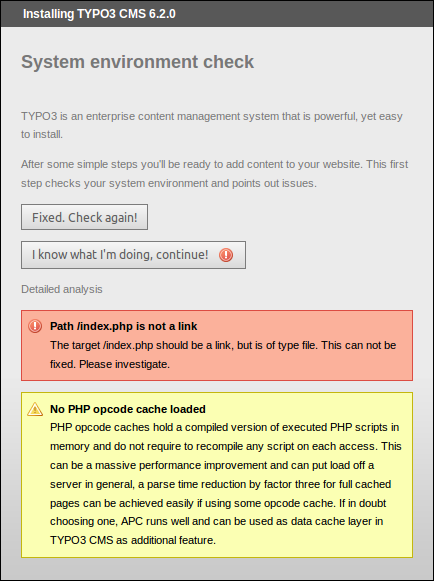
\includegraphics[width=0.8\linewidth]{Images/InstallTool/SystemEnvironmentCheck.png}
			\end{figure}
		\end{column}

	\end{columns}

\end{frame}

% ------------------------------------------------------------------------------
% Re-Development
% ------------------------------------------------------------------------------

\begin{frame}[fragile]
	\frametitle{Install Tool}
	\framesubtitle{Neu-Entwicklung}

	\begin{columns}[T]

		\begin{column}{.5\textwidth}
			\begin{itemize}
				\item Im \underline{zweiten} Schritt werden die Zugangsdaten zum Datenbank-\newline
					server angegeben
				\item Verschiedene Verbindungstypen können ausgewählt werden
					\begin{itemize}
						\item TCP/IP Verbindung
						\item Socket Verbindung
					\end{itemize}
				\item Alternativen zu MySQL sind ebenfalls möglich
			\end{itemize}
		\end{column}

		\begin{column}{.5\textwidth}
			\begin{figure}\vspace*{-0.4cm}
				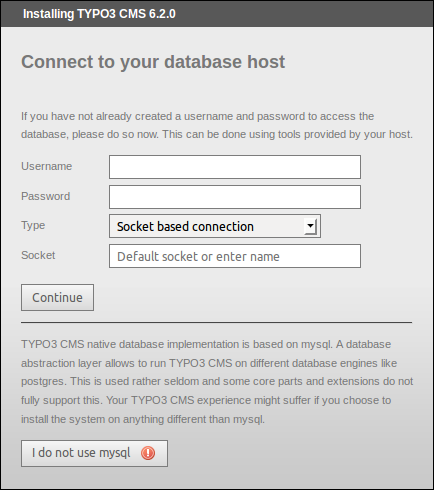
\includegraphics[width=0.8\linewidth]{Images/InstallTool/DatabaseConnectionDetails.png}
			\end{figure}
		\end{column}

	\end{columns}

\end{frame}

% ------------------------------------------------------------------------------
% Re-Development
% ------------------------------------------------------------------------------

\begin{frame}[fragile]
	\frametitle{Install Tool}
	\framesubtitle{"Neu-Entwicklung}

	\begin{columns}[T]

		\begin{column}{.5\textwidth}
			\begin{itemize}
				\item Der \underline{dritte} Schritt erlaubt es, die Datenbank auszuwählen oder zu erstellen (wie bereits in Versionen vor TYPO3 6.2)
				\item Im \underline{vierten} Schritt wird das Passwort für den Benutzer "admin" gesetzt (welches ebenso das Install Tool Passwort darstellt) und der Sitename angegeben
			\end{itemize}
		\end{column}

		\begin{column}{.5\textwidth}
			\begin{figure}\vspace*{-0.4cm}
				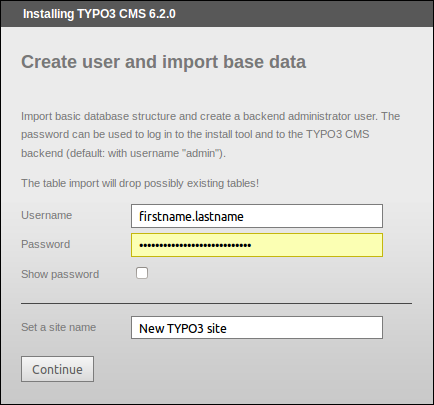
\includegraphics[width=0.8\linewidth]{Images/InstallTool/AdminPasswordAndSiteName.png}
			\end{figure}
		\end{column}

	\end{columns}

\end{frame}

% ------------------------------------------------------------------------------
% Delete All Cache
% ------------------------------------------------------------------------------

\begin{frame}[fragile]
	\frametitle{Install Tool}
	\framesubtitle{Cache vollständig leeren}

	\begin{itemize}
		\item Mit einer neuen Funktion unter "Important actions" kann der gesamte Cache vollständig geleert werden ("Delete all cache")
		\item Jenes funktioniert auch, wenn der Cache ungültigen PHP Code enthält, der möglicherweise TYPO3 blockiert
		\item Um eine nicht-funktionierende TYPO3 Instanz zu umgehen, kann das Install Tool direkt aufgerufen werden: \texttt{http://example.com/typo3/install}
	\end{itemize}

	\begin{columns}[T]
		\begin{column}{.3\textwidth}
			\begin{figure}\vspace*{-0.4cm}
				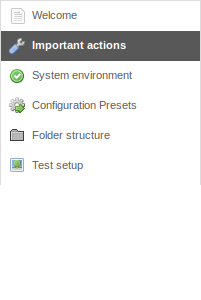
\includegraphics[width=0.7\linewidth]{Images/InstallTool/ImportantActionsCropped1.png}
			\end{figure}
		\end{column}
		\begin{column}{.7\textwidth}
			\begin{figure}\vspace*{-0.4cm}
				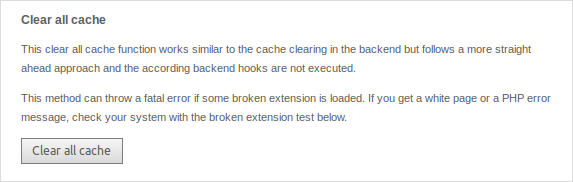
\includegraphics[width=0.9\linewidth]{Images/InstallTool/ClearAllCache.png}
			\end{figure}
		\end{column}
	\end{columns}

\end{frame}

% ------------------------------------------------------------------------------
% Delete All Cache
% ------------------------------------------------------------------------------

\begin{frame}[fragile]
	\frametitle{Install Tool}
	\framesubtitle{Cache vollständig leeren}

	Ablauf, wenn die Funktion "Delete all cache" ausgeführt wird:

	\begin{enumerate}
		\item Inhalt des Verzeichnisses \texttt{typo3temp/Cache} wird gelöscht
		\item Datenbanktabellen \texttt{cf\_*} werden geleert
		\item Dateien \texttt{ext\_localconf.php} und \texttt{ext\_tables.php}\newline
			von installierten Extensions werden geladen
		\item \texttt{flushCaches()} wird ausgeführt
	\end{enumerate}

\end{frame}

% ------------------------------------------------------------------------------
% Check For Broken Extensions
% ------------------------------------------------------------------------------

\begin{frame}[fragile]
	\frametitle{Install Tool}
	\framesubtitle{Nicht-ausführbare Extensions}

	\begin{itemize}
		\item Mit einer neuen Funktion unter "Important actions" kann nun geprüft werden, ob Extensions geladen werden können, ohne das System lahm zu legen
		\item Sehr nützlich zum Beispiel bei einem Update von TYPO3 4.5 zu 6.2
	\end{itemize}

	\begin{columns}[T]
		\begin{column}{.3\textwidth}
			\begin{figure}\vspace*{-0.4cm}
				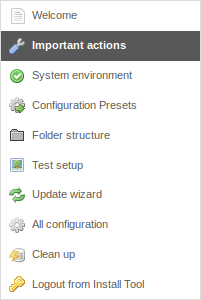
\includegraphics[width=0.7\linewidth]{Images/InstallTool/ImportantActions.png}
			\end{figure}
		\end{column}
		\begin{column}{.7\textwidth}
			\begin{figure}\vspace*{-0.4cm}
				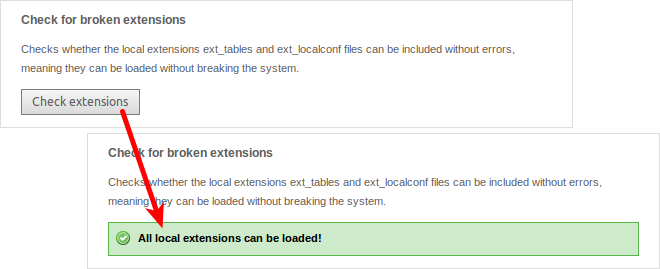
\includegraphics[width=1\linewidth]{Images/InstallTool/CheckForBrokenExtensions.png}
			\end{figure}
		\end{column}
	\end{columns}

\end{frame}

% ------------------------------------------------------------------------------
% Increased Security: Salted Passwords
% ------------------------------------------------------------------------------

\begin{frame}[fragile]
	\frametitle{Install Tool}
	\framesubtitle{Gesalzene Passwörter}

	\begin{itemize}
		\item Beim Neuerstellen von Administratorkonten über das Install Tool, werden nun \textbf{gesalzene} (salted) Passwörter verwendet\newline
			\smaller(vorausgesetzt, EXT:saltedpasswords ist installiert und konfiguriert)\normalsize
		\item Das Install Tool Passwort ist ebenfalls ein \textbf{gesalzenes} Passwort\newline
			\smaller(ein existierender MD5 Hash wird beim ersten Login umgewandelt)\normalsize
	\end{itemize}

	\begin{columns}[T]
		\begin{column}{.3\textwidth}
			\begin{figure}\vspace*{-0.4cm}
				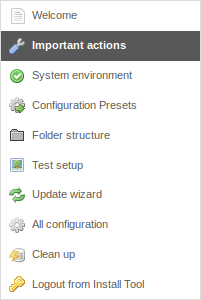
\includegraphics[width=0.7\linewidth]{Images/InstallTool/ImportantActions.png}
			\end{figure}
		\end{column}
		\begin{column}{.7\textwidth}
			\begin{figure}\vspace*{-0.4cm}
				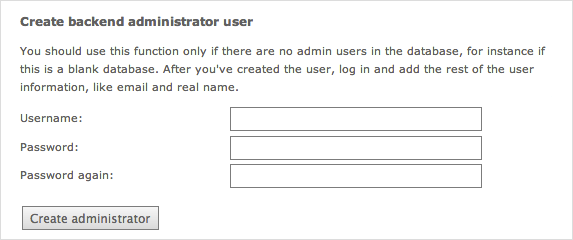
\includegraphics[width=0.9\linewidth]{Images/InstallTool/SaltedPasswords.png}
			\end{figure}
		\end{column}
	\end{columns}

\end{frame}

% ------------------------------------------------------------------------------
% Application Context
% ------------------------------------------------------------------------------

\begin{frame}[fragile]
	\frametitle{Install Tool}
	\framesubtitle{Application Context (1)}

	\begin{itemize}
		\item TYPO3 ab Version 6.2 berücksichtigt nun den \textbf{Application Context}\newline
			\smaller(bereits bekannt von TYPO3 Flow)\normalsize
		\item Umgebungsvariable \texttt{TYPO3\_CONTEXT} setzt diesen Kontext\newline
			\smaller(Voreinstellung: \texttt{Production}, Sub-Context wie z.B. \texttt{Production/Staging} möglich)\normalsize

			\begin{lstlisting}
				# File: .htaccess
				# Rules to set Application Context based on hostname:

				RewriteCond %{HTTP_HOST} ^dev\.example\.com$
				RewriteRule (.*) $1 [E=TYPO3_CONTEXT:Development]

				RewriteCond %{HTTP_HOST} ^www\.example\.com$
				RewriteRule (.*) $1 [E=TYPO3_CONTEXT:Production]

				# Sets an environment variable, which is then available to TYPO3 CMS:
				SetEnv TYPO3_CONTEXT Production
			\end{lstlisting}

	\end{itemize}

\end{frame}

% ------------------------------------------------------------------------------
% Presets of TYPO3_CONF_VAR Settings
% ------------------------------------------------------------------------------

\begin{frame}[fragile]
	\frametitle{Install Tool}
	\framesubtitle{Vorkonfigurierte TYPO3\_CONF\_VAR Einstellungen}

	\begin{columns}[T]
		\begin{column}{.5\textwidth}

			\begin{itemize}
				\item Vorkonfigurierte \texttt{TYPO3\_CONF\_VAR}-Einstellungen können im Install Tool ausgewählt werden
				\item Diverse Parameter steuern zum Beispiel Debug-Ausgaben, das "deprecation log", devIPmask und weitere Log-Einstellungen
				\item Vorgegebene Kontexte sind "Production" and "Development"\newline
					(eine eigene Konfiguration ist natürlich möglich)
			\end{itemize}

		\end{column}
		\begin{column}{.5\textwidth}

			\begin{figure}\vspace*{-0.4cm}
				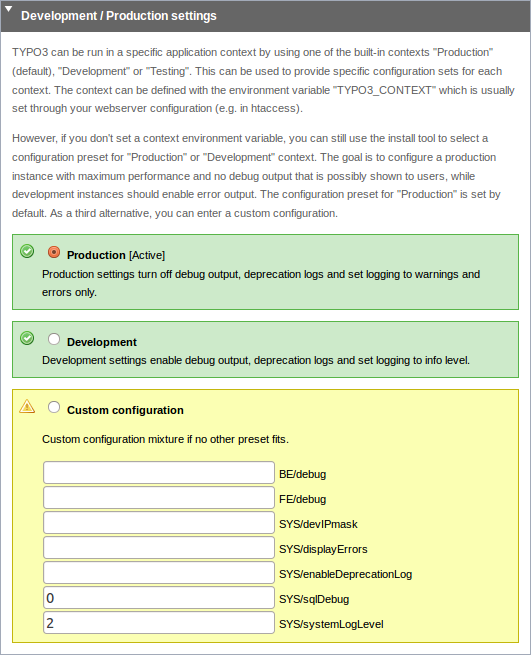
\includegraphics[width=0.8\linewidth]{Images/InstallTool/PresetsOfSettings.png}
			\end{figure}

		\end{column}
	\end{columns}

\end{frame}

% ------------------------------------------------------------------------------
% Improved Usability
% ------------------------------------------------------------------------------

\begin{frame}[fragile]
	\frametitle{Install Tool}
	\framesubtitle{Verbesserte Benutzerfreundlichkeit}

	\begin{columns}[T]
		\begin{column}{.5\textwidth}

			\begin{itemize}
				\item Die Position des Menüs auf der linken Seite ist nun fixiert und das Menü scrollt nicht mit
				\item Der Button "Write configuration" am Ende der Seite ist fixiert und somit immer sichtbar
				\item Einträge in "All Configuration" sind gruppiert (klappen bei Klick auf die Überschrift auf)
			\end{itemize}

		\end{column}
		\begin{column}{.5\textwidth}

			\begin{figure}\vspace*{-0.4cm}
				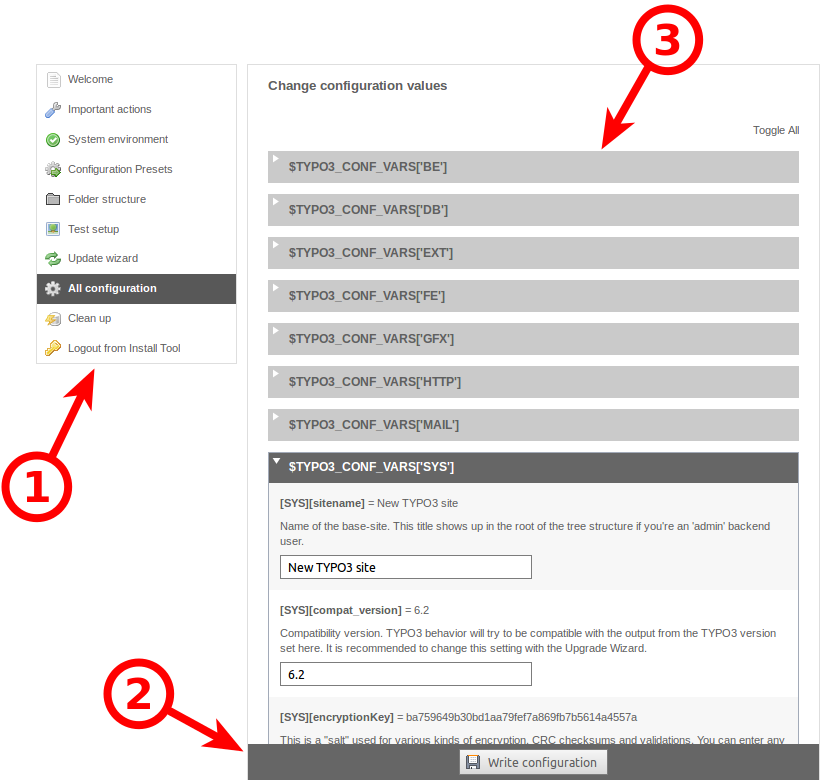
\includegraphics[width=0.8\linewidth]{Images/InstallTool/ImprovedUsability.png}
			\end{figure}

		\end{column}
	\end{columns}

\end{frame}

% ------------------------------------------------------------------------------
% Human-Friendly Error Codes
% ------------------------------------------------------------------------------

\begin{frame}[fragile]
	\frametitle{Install Tool}
	\framesubtitle{Benutzerfreundliche Fehlercodes}

	\begin{itemize}
		\item Aussagekräftige (menschen-lesbare) Begriffe können für folgende Optionen verwendet werden:
	\end{itemize}

	\begin{columns}[T]
		\begin{column}{.4\textwidth}
			\advance\leftskip+0.8cm

			\smaller
				\texttt{[SYS][errorHandlerErrors]}\newline
				\texttt{[SYS][exceptionalErrors]}\newline
				\texttt{[SYS][syslogErrorReporting]}\newline
				\texttt{[SYS][belogErrorReporting]}\newline
			\normalsize

			\small(vor TYPO3 6.2 waren nur numerische Werte möglich)\normalsize

		\end{column}
		\begin{column}{.6\textwidth}

			\begin{figure}\vspace*{-0.4cm}
				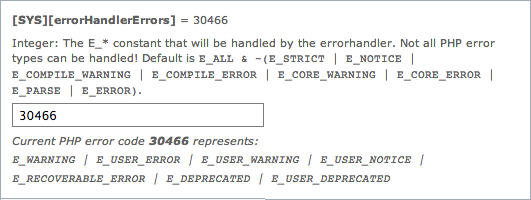
\includegraphics[width=0.9\linewidth]{Images/InstallTool/HumanFriendlyErrorCodes.png}
			\end{figure}

		\end{column}
	\end{columns}

	\vspace{0.2cm}

	\begin{itemize}
		\item Ein Extbase ViewHelper \textbf{format.phpErrorCode} übernimmt die Umwandlung in PHP Fehlercodes
	\end{itemize}

\end{frame}

% ------------------------------------------------------------------------------
% Errors In Folder Structure
% ------------------------------------------------------------------------------

\begin{frame}[fragile]
	\frametitle{Install Tool}
	\framesubtitle{Verzeichnis-Fehler}

	\begin{itemize}
		\item Fehler in der Verzeichnisstruktur werden direkt angezeigt\newline
			(als "Badge", eingekreiste Zahl)
	\end{itemize}

	\begin{figure}
		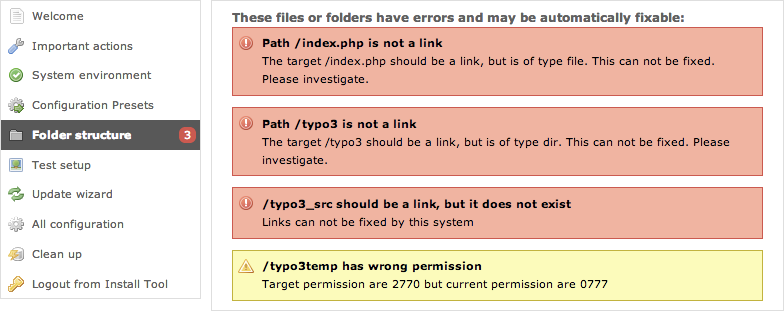
\includegraphics[width=0.95\linewidth]{Images/InstallTool/ErrorsInFolderStructure.png}
	\end{figure}

\end{frame}

% ------------------------------------------------------------------------------
% Core Updates
% ------------------------------------------------------------------------------

\begin{frame}[fragile]
	\frametitle{Install Tool}
	\framesubtitle{TYPO3 Core Updates}

	\begin{itemize}
		\item Minor-Core-Updates (inkl. Security-Versionen) können direkt aus dem Install Tool ausgeführt werden
		\item Die Umgebungsvariable \texttt{TYPO3\_DISABLE\_CORE\_UPDATER=1} unterbindet diese Funktion
	\end{itemize}

	\begin{figure}
		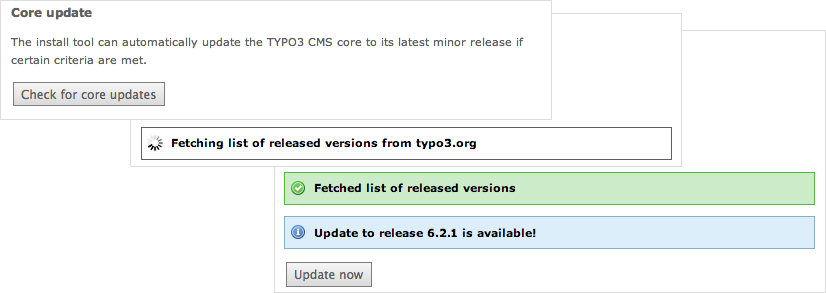
\includegraphics[width=0.9\linewidth]{Images/InstallTool/CoreUpdate.png}
	\end{figure}

\end{frame}

% ------------------------------------------------------------------------------
% Miscellaneous
% ------------------------------------------------------------------------------

\begin{frame}[fragile]
	\frametitle{Install Tool}
	\framesubtitle{Diverses}

	\begin{itemize}
		\item Sämtliche Formulare sind nun CSRF-geschützt\newline
			\smaller(\textit{cross-site request forgery})\normalsize
		\item Das Install Tool nutzt einen vereinfachten Fluid Standalone View
		\item Nur unbedingt notwendige TYPO3 Funktionen werden geladen\newline
			\small(Extensions mit beschädigten \texttt{ext\_localconf.php} oder \texttt{ext\_tables.php} Dateien führen nicht mehr zum Abbruch des Install Tools)\normalsize
		\item Neuer Startpunkt:	\tabto{3.2cm} \texttt{typo3/sysext/install/Start/Install.php}\newline
			War bisher:			\tabto{3.2cm} \texttt{typo3/install/index.php}\newline
			\small(es existiert eine Umleitung von der alten zur neuen Adresse)\normalsize
		\item Damit das Install Tool auch benutzbar bleibt, wenn der Cache ungültigen PHP Code enthält, verzichtet es komplett auf Caching
	\end{itemize}

\end{frame}

% ------------------------------------------------------------------------------
% Miscellaneous
% ------------------------------------------------------------------------------

\begin{frame}[fragile]
	\frametitle{Install Tool}
	\framesubtitle{Diverses}

	\begin{itemize}
		\item Es wird geprüft, ob die PHP Option \texttt{xdebug.max\_nesting\_level} einen Wert von mindestens 250 aufweist\newline
			\small(die Voreinstellung "100" führt unter Umständen zu Fehlern)\normalsize
		\item "Relaxed permission check":

			\small
				Während normalerweise die Berechtigung für das Root-Verzeichnis der Installation
				2770 sein muss und der Ordner dem Web-User gehören muss, um TYPO3 zu installieren,
				wurde nun eine Option "targetPermissionRelaxed" eingeführt, bei der dieser Check
				für den Root-Folder außer Kraft gesetzt wurde, sofern es trotzdem möglich ist,
				die benötigten Unterverzeichnisse anzulegen.
			\normalsize

	\end{itemize}

\end{frame}

% ------------------------------------------------------------------------------
% Miscellaneous
% ------------------------------------------------------------------------------

\begin{frame}[fragile]
	\frametitle{Install Tool}
	\framesubtitle{Diverses}

	\begin{itemize}
		\item Folgende veraltete Optionen wurden vom Install Tool entfernt\newline
			(und damit auch aus der Datei \texttt{LocalConfiguration.php}):
	\end{itemize}

	\begin{columns}[T]
		\begin{column}{.5\textwidth}
			\advance\leftskip+0.8cm
			\smaller
				\texttt{BE/loginLabels}\newline
				\texttt{BE/loginNews}\newline
				\texttt{BE/useOnContextMenuHandler}\newline
				\texttt{EXT/em\_mirrorListURL}\newline
				\texttt{EXT/em\_wsdlURL}\newline
				\texttt{EXT/extList}\newline
				\texttt{EXT/extList\_FE}\newline
				\texttt{EXT/noEdit}\newline
			\normalsize
		\end{column}
		\begin{column}{.5\textwidth}
			\smaller
				\texttt{FE/defaultTypoScript\_editorcfg}\newline
				\texttt{FE/simulateStaticDocuments}\newline
				\texttt{GFX/noIconProc}\newline
				\texttt{GFX/TTFLocaleConv}\newline
				\texttt{SYS/additionalAllowedClassPrefixes}\newline
				\texttt{SYS/caching/cacheBackends}\newline
				\texttt{SYS/caching/cacheFrontends}\newline
				\texttt{SYS/extCache}\newline
				\texttt{SYS/T3instID}\newline
			\normalsize
		\end{column}
	\end{columns}

\end{frame}

% ------------------------------------------------------------------------------

